\documentclass{article}
\usepackage[utf8]{inputenc}
\usepackage[frenchb]{babel}
\usepackage[T1]{fontenc}
\usepackage{authblk}
\usepackage{hyperref}
\usepackage{fancyhdr}
\usepackage{titling}
\usepackage{graphicx}
\usepackage{geometry}
\usepackage{enumitem}
\usepackage{microtype}
\usepackage[none]{hyphenat}
\usepackage[toc]{glossaries}
\makeglossaries

\newacronym{REST}{REST}{transfert d'état représentationnel}


 \geometry{
 a4paper,
 total={169mm,240mm},
 left=16mm,
 top=20mm,
 }

\usepackage{listings} % For code coloration
\usepackage{color}
\usepackage[dvipsnames]{xcolor}


\definecolor{codegreen}{rgb}{0,0.6,0}
\definecolor{codegray}{rgb}{0.5,0.5,0.5}
\definecolor{codepurple}{rgb}{0.58,0,0.82}
\definecolor{backcolour}{rgb}{0.95,0.95,0.92}


\headheight = 14pt

\hypersetup{colorlinks = true,citecolor=black,filecolor=black,linkcolor=black,urlcolor=black}

\lstdefinestyle{s}{
  backgroundcolor=\color{backcolour},   commentstyle=\color{codegreen},
  keywordstyle=\color{NavyBlue},
  numberstyle=\tiny\color{codegray},
  stringstyle=\color{codepurple},
  basicstyle=\footnotesize,
  breakatwhitespace=false,         
  breaklines=true,                 
  captionpos=b,                    
  keepspaces=true,                 
  numbers=left,                    
  numbersep=5pt,                  
  showspaces=false,                
  showstringspaces=false,
  showtabs=false,                  
  tabsize=4
}


\lstset{style=s}
\lstset{literate=
  {á}{{\'a}}1 {é}{{\'e}}1 {í}{{\'i}}1 {ó}{{\'o}}1 {ú}{{\'u}}1
  {Á}{{\'A}}1 {É}{{\'E}}1 {Í}{{\'I}}1 {Ó}{{\'O}}1 {Ú}{{\'U}}1
  {à}{{\`a}}1 {è}{{\`e}}1 {ì}{{\`i}}1 {ò}{{\`o}}1 {ù}{{\`u}}1
  {À}{{\`A}}1 {È}{{\'E}}1 {Ì}{{\`I}}1 {Ò}{{\`O}}1 {Ù}{{\`U}}1
  {ä}{{\"a}}1 {ë}{{\"e}}1 {ï}{{\"i}}1 {ö}{{\"o}}1 {ü}{{\"u}}1
  {Ä}{{\"A}}1 {Ë}{{\"E}}1 {Ï}{{\"I}}1 {Ö}{{\"O}}1 {Ü}{{\"U}}1
  {â}{{\^a}}1 {ê}{{\^e}}1 {î}{{\^i}}1 {ô}{{\^o}}1 {û}{{\^u}}1
  {Â}{{\^A}}1 {Ê}{{\^E}}1 {Î}{{\^I}}1 {Ô}{{\^O}}1 {Û}{{\^U}}1
  {œ}{{\oe}}1 {Œ}{{\OE}}1 {æ}{{\ae}}1 {Æ}{{\AE}}1 {ß}{{\ss}}1
  {ű}{{\H{u}}}1 {Ű}{{\H{U}}}1 {ő}{{\H{o}}}1 {Ő}{{\H{O}}}1
  {ç}{{\c c}}1 {Ç}{{\c C}}1 {ø}{{\o}}1 {å}{{\r a}}1 {Å}{{\r A}}1
  {€}{{\EUR}}1 {£}{{\pounds}}1 {°}{{\no}}1
}

\pretitle{
  \begin{center}
  
\includegraphics[width=60mm,height=31mm]{img/univ.png}
  \qquad \qquad
  
\includegraphics[width=37mm,height=31mm]{img/iutNantes.jpg}\\[\bigskipamount]
}
 
\posttitle{
 \end{center}
}
  
\title{Back End marketing conversationnel\\
    \normalsize Technologies web côté serveur}
\date{\today}
\author{Paul Orhon\\
\small LP -- MiAR -- Université de Nantes }

\pagestyle{fancy}
\fancyhf{}
\rhead{Paul Orhon --- \small LP -- MiAR}
\lhead{Marketing conversationnel --- Technologies web côté serveur}
\rfoot{Page \thepage}
\lfoot{INSTITUT UNIVERSITAIRE DE TECHNOLOGIE - NANTES}


\begin{document}

\maketitle%page titre
\tableofcontents


\listoffigures


\clearpage

\section{Projet}
Ce projet a pour but de développer le Back End d’un marketing conversationnel.
Pour cela il faut développer différent service pour pouvoirs mettre en place ce système.

Voici le workflow classique d'un utilisateur:\\
\begin{figure}[h]
    \centering
    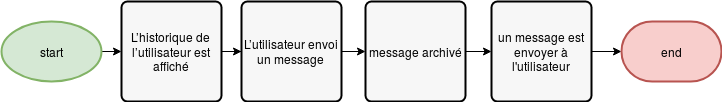
\includegraphics[width=\linewidth]{img/workflow_user.png}
    \caption{Workflow classique d'un utilisateur}
\end{figure}



\section{Contexte du projet}
\subsection{Objectifs}
L’objectif est de développer le Back End d’un marketing conversationnel, en exposant les service avec une api \acrshort{REST}*.

Toute les conversations doivent être conservées pour pouvoir effectuer des statistiques.

Le projet doit être séparer en sous module, permettant de manipuler, modifier et diffuser plus facilement.


\subsection{Contraintes}
\begin{enumerate}
    \item Le projet est à réalisé seul.
    \item Le programme sera développé pour la plateforme Java.
    \begin{itemize}
        \item Il sera programmé en Java pour des raisons de connaissance.
    \end{itemize}
    \item Le rapport est à rendre le 20 novembre 2017 à 17h50.
    \item Le projet est à rendre le 5 décembre 2017 à 12h20.
    \item le système doit être testé, testable et le couplage doit être lâche.
\end{enumerate}


\section{Les vues}
\subsection{Vue globale du projet}

\begin{figure}[h]
    \centering
    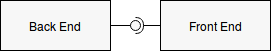
\includegraphics[]{img/Diagramme_sep_Back_Front.png}
    \caption{Diagramme de la séparation du Back / Front End}
    \label{fig:diag_back_front}
\end{figure}
Comme dit précédemment, seule le back end et son interface sera développer (partie en rouge de la figure \ref{fig:diag_back_front}).

\clearpage
\subsection{Vue logique du Back End}
Le back end sera diviser en plusieurs modules permettent ainsi de diviser les tâches, de réaliser un couplage lâche et de faciliter le maintien du système.
\begin{figure}[h]
    \centering
    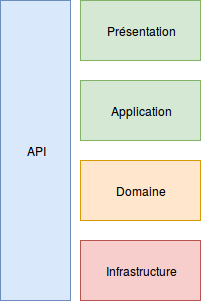
\includegraphics[]{img/Vue_logique_back.png}
    \caption{Diagramme de la vue logique du backEnd}
\end{figure}

Ici chaque couleur correspond à un module.

\begin{description}
    \item [Application] qui contient aussi la Présentation du fait de l'utilisation du framework Spring qui permet une mise en place simple d'une api \acrshort{REST} et donc de l'interface du back end. Sont rôle est de récupérer les requête arrivant a l'interface, de les envoyer au bon service et de répondre.
    \item [Domaine] correspond au \textit{services} de l’application.
    \item [Infrastructure] correspond à l'implémentassions des différentes              \textbf{\textit{interface}} et \textbf{\textit{class abstraites}}.
    \item [API] contient les \textbf{\textit{interface}} des class communes aux modules. Cela permet notamment au \textbf{domaine} d'utiliser une class et de laisser l'implémentassions à l'\textbf{Infrastructure}.
\end{description}

projection

intéret des couches


\clearpage
\printglossary[type=\acronymtype, title=Acronymes]

\end{document}
    